\chapter{System identification}
\label{identification_design}

\emph{In this chapter, the Multi-inlet, Multi-WT model, which has been derived based on first principles in \chapref{system_modelling}, is reformulated such that it is suitable for system identification. First, the structure of the model is discussed, then a Neural Network(NN) based identification method is presented. In the first case, the identification is tested on a simple example, then on the Randers EPANET WSS model. In the second case, the identification is carried out based on measurements from the real-world network.}

\section{Model structure of the Multi-inlet, Multi-WT system}
\label{model_structure_of_the_multi_inlet_multi_WT_system}

In \chapref{system_modelling}, the model of a multi-inlet WSS with the extension of multiple WTs has been derived. The network has been represented by a non-linear State Space model, which includes the equations describing the dynamics, the outputs and the equations describing a constraint on certain flows in the network. As the derivation of the model has been carried out based on first principles, insight has been given into the structure and between all the describing physical variables. 

\subsection{Output equation}
\label{output_eq_identification}

In order to utilize the presented model for control, identification is required. For identification purposes, the non-linear State Space representation of the system is going to be used, therefore let us recall the governing equations. The output vector describes the inlet pressure $\bar{p}_{\mathcal{K}}$ which is given in discrete form such that

\begin{equation}
  \label{recall_output_eq}
  \bar{p}^{k}_{\mathcal{K}} = K^T \bar{H}^{-T}_{\mathcal{T}}f_{\mathcal{T}}(A_2 q^{k}_{\mathcal{C}} + A_3 K \bar{d}^{k}_{\mathcal{K}} - A_3 D v_{\mathcal{D}} \sigma^{k}) - K^T\bar{H}^{-T}_{\mathcal{T}}\hat{H}^{T}_{\mathcal{T}} (\hat{p}^{k} + \hat{h}) - K^T\bar{h} ,
\end{equation} 

\vspace{-1mm}

\begin{minipage}[t]{0.4\textwidth}
where\\
\hspace*{8mm} $A_2 = -\bar{H}^{-1}_{\mathcal{T}} \bar{H}_{\mathcal{C}} $, \vspace*{1.5mm}\\
\hspace*{8mm} $A_3 = \bar{H}^{-1}_{\mathcal{T}}$.
\end{minipage}

and furthermore, $\bar{d}^{k}_{\mathcal{K}}$ inlet flows, $\sigma^{k}$ total demand, $v_{\mathcal{D}}$ distribution parameter, $q^{k}_{\mathcal{C}}$ flows in set $\mathcal{C}$, $\hat{p}^{k}$ pressures in the WTs, $\hat{h}$ elevations of the WTs and $K^T\bar{h} = \bar{h}_{\mathcal{K}} $ the elevations of the pumping stations. The corresponding values of the pressures and flows in the network are evaluated at each time step $k$. 

Additionally, let us recall the constraint on $q_\mathcal{C}$, and rewrite it in discrete-time form such that

 \begin{equation}
\label{recall_constraint eq}
f_{\mathcal{C}}(q^{k}_{\mathcal{C}}) - A_1(\hat{p}^{k} + \hat{h}) + A_2^T f_{\mathcal{T}}(A_2 q^{k}_{\mathcal{C}} + A_3 K \bar{d}^{k}_{\mathcal{K}} - A_3 D v_{\mathcal{D}} \sigma^{k}) = 0.
\end{equation} 

\vspace{-1mm}

\begin{minipage}[t]{0.4\textwidth}
where\\
\hspace*{8mm} $A_1 = \hat{H}^T_{\mathcal{C}} -\bar{H}^T_{\mathcal{C}}\bar{H}^{-T}_{\mathcal{T}}\hat{H}^T_{\mathcal{T}}$. 
\end{minipage}

It is important to point out that the model in \chapref{system_modelling} has been derived in a general manner, taking into account that $v_{\mathcal{D}}$ is a time-varying distribution parameter of the demands. However, in the further description, let us restrict ourselves and assume that $v_{\mathcal{D}}$ is constant.  From the technical point of view, the identification becomes less complex, as in this case $v_{\mathcal{D}}$ is a linear constant parameter. Furthermore, there is no need to introduce $v_{\mathcal{D}}$ as a time-varying parameter on the EPANET data, however on the real measurement data, the possible demand variations might be experienced. In \eqref{recall_constraint eq} and \eqref{recall_output_eq} the assumption of $v_{\mathcal{D}}$ being constant is already taken into account, therefore $v_{\mathcal{D}}$ does not have any time index.

% This assumption is beneficial from the system point of view, as the total consumption $\sigma_k$ can be represented simply by the sum of the hourly demand variations $1^T \bar{d}_{\mathcal{D}}$. 

The constraint on $q^{k}_{\mathcal{C}}$ in \eqref{recall_constraint eq} is given by an implicit expression for which an analytical solution has not been derived. The explicit solution for the constraint has a structure like \eqref{qc_abstraction}, however we do not know how it looks exactly.

 \begin{equation}
\label{qc_abstraction}
q^{k}_{\mathcal{C}} = q_{\mathcal{C}} \big( (\hat{p}^{k} + \hat{h}),\bar{d}^{k}_{\mathcal{K}}, \sigma^{k} \big).
\end{equation} 

It is shown in \eqref{qc_abstraction} that the $q^{k}_{\mathcal{C}}$ flows in the network depend on the same physical measures, i.e. the same variables as the outputs $\bar{p}^{k}_{\mathcal{K}}$. By substituting \eqref{qc_abstraction} into \eqref{recall_output_eq}, we get the following output equation

\vspace{-4mm}
\begin{align}
  \label{recall_output_eq_2}
      \bar{p}^{k}_{\mathcal{K}}  = & \nonumber K^T \bar{H}^{-T}_{\mathcal{T}}f_{\mathcal{T}} \big (A_2 q_{\mathcal{C}}\big ((\hat{p}^{k} + \hat{h}),\bar{d}^{k}_{\mathcal{K}}, \sigma^{k} \big) + A_3 K \bar{d}^{k}_{\mathcal{K}} - A_3 D v_{\mathcal{D}} \sigma^{k} \big)   \\ &  - K^T\bar{H}^{-T}_{\mathcal{T}}\hat{H}^{T}_{\mathcal{T}} (\hat{p}^{k} + \hat{h}) - \bar{h}_{\mathcal{K}} .
\end{align}

\vspace{-4mm}
In \eqref{recall_output_eq_2}, the pressure head in the pumping stations $\bar{p}^{k}_{\mathcal{K}}$ is given by the expression on the right-hand side. Let us write \eqref{recall_output_eq_2} in a form where the non-linear expression on the right-hand side is replaced with a non-linear function $\tilde{f}_1(\cdot)$, which has an unknown structure but has the same variables in the argument. Thus, the reformulated output equation is given such that 

 \begin{equation}
  \label{recall_output_eq_3}
     \bar{p}^{k}_{\mathcal{K}}  = \tilde{f}_1 \big((\hat{p}^{k} + \hat{h}),\bar{d}^{k}_{\mathcal{K}}, \sigma^{k}\big) + \tilde{a}_{\mathcal{K}} (\hat{p}^{k} + \hat{h}) - \bar{h}_{\mathcal{K}}, 
\end{equation} 

\vspace{-1mm}

\begin{minipage}[t]{0.4\textwidth}
where\\
\hspace*{8mm} $\tilde{a}_{\mathcal{K}} = - K^T\bar{H}^{-T}_{\mathcal{T}}\hat{H}^{T}_{\mathcal{T}} $. 
\end{minipage}

The output equation described in \eqref{recall_output_eq_3} is a mapping defined by the non-linear function $\tilde{f}_1$ and the remaining linear terms, which map the input set, $u^{k} = ( \hat{p}^{k}\!+\!\hat{h} \ \bar{d}^{k}_{\mathcal{K}} \ \sigma^{k} )^T$ to the outputs $\bar{p}^{k}_{\mathcal{K}}$. 

Typically, the pressure is measured in the WTs not the total head, therefore the elevation $\bar{h}_{\mathcal{K}}$ is not added to $\bar{p}^{k}_{\mathcal{K}}$, although in some cases it can be assumed to be known. In the input set, the total consumption can be calculated according to the mass-balance in the network such that

\begin{equation}
\label{massbalance_identification}
 \sigma^{k} = 1^T \hat{d}^{k} + 1^T \bar{d}^{k}_{\mathcal{K}}.
\end{equation}

 In \eqref{massbalance_identification}, we assume that the flows in the WTs are measured, as the demand flows $\bar{d}^{k}_{\mathcal{D}} $ are not measurable. 

 \subsection{State equation}
\label{state_eq_identification} 

The state equation is a first-order system of ODEs, which has been formulated on the pressures $\hat{p}$ in the WTs. In order to give the discrete form of the approximate solution of the ODEs, Euler-method is used. The Euler-method is the simplest Runge-Kutta method, which provides an acceptable precision for our problem\cite{chicone2006ordinary}. Thus, the discrete state equation yields

\begin{equation}
  \label{WT_matrixform_final_discrete}
\Lambda \frac{1}{T_s} (\hat{p}^{(k+1)} - \hat{p}^{k})  = - (\hat{H}_{\mathcal{C}} - \hat{H}_{\mathcal{T}} \bar{H}^{-1}_{\mathcal{T}}\bar{H}_{\mathcal{C}})  q^{k}_{\mathcal{C}} - \hat{H}_{\mathcal{T}} \bar{H}^{-1}_{\mathcal{T}} K \bar{d}^{k}_{\mathcal{K}} + \hat{H}_{\mathcal{T}} \bar{H}^{-1}_{\mathcal{T}} D v_{\mathcal{D}} \sigma^{k}.
\end{equation}

\begin{minipage}[t]{0.20\textwidth}
where\\
\hspace*{8mm} $T_s$
\end{minipage}
\begin{minipage}[t]{0.68\textwidth}
\vspace*{2mm}
 is the sampling time.
\end{minipage}
\begin{minipage}[t]{0.10\textwidth}
\vspace*{2mm}
\textcolor{White}{te}$\unit{h}$
\end{minipage} 

Substituting the constraint on $q_{\mathcal{C}}$ into \eqref{WT_matrixform_final_discrete}, and expressing the predicted values of the WT pressures on the left-hand side, the following can be written

\vspace{-4mm}
\begin{align}
\label{WT_matrixform_final_discrete1}
\nonumber  \hat{p}^{(k+1)}  =& T_s \Lambda^{-1} \big(- (\hat{H}_{\mathcal{C}} - \hat{H}_{\mathcal{T}} \bar{H}^{-1}_{\mathcal{T}}\bar{H}_{\mathcal{C}})  q^{k}_{\mathcal{C}}\big ((\hat{p}^{k} + \hat{h}),\bar{d}^{k}_{\mathcal{K}}, \sigma^{k} \big) \\ & - \hat{H}_{\mathcal{T}} \bar{H}^{-1}_{\mathcal{T}} K \bar{d}^{k}_{\mathcal{K}} + \hat{H}_{\mathcal{T}} \bar{H}^{-1}_{\mathcal{T}} D v_{\mathcal{D}} \sigma^{k} \big) + \hat{p}^{k} .
\end{align}
\vspace{-4mm}


\eqref{WT_matrixform_final_discrete} describes the relation between the flows $q^{k}_{\mathcal{C}}$, the total head in the WTs $(\hat{p}^{k} + \hat{h})$ and the total consumption $\sigma^{k}$. However, by substituting the $q^{k}_{\mathcal{C}}$ flows with their non-linear expression, the structure of the state equation is not a linear combination of the corresponding signals anymore. Therefore, let us write \eqref{WT_matrixform_final_discrete1} in a form where the non-linear terms are described by a non-linear function $\tilde{f}_2(\cdot)$ with unknown structure, similarly as it has been done for the output equation. Thus, the reformulated state equation can be given such that

 \begin{equation}
  \label{WT_matrixform_final_discrete2}
     \hat{p}^{(k+1)}  = \tilde{f}_2 \big((\hat{p}^{k} + \hat{h}),\bar{d}^{k}_{\mathcal{K}}, \sigma^{k}\big) + \tilde{a}_{\mathcal{W}} \bar{d}^{k}_{\mathcal{K}} + \tilde{b}_{\mathcal{W}} \sigma^{k} + \hat{p}^{k},
\end{equation}

\vspace{-1mm} 

\begin{minipage}[t]{0.4\textwidth}
where\\
\hspace*{8mm} $\tilde{a}_{\mathcal{W}} = - \hat{H}_{\mathcal{T}} \bar{H}^{-1}_{\mathcal{T}} K $, \vspace*{1.5mm}\\
\hspace*{8mm} $\tilde{b}_{\mathcal{W}} = \hat{H}_{\mathcal{T}} \bar{H}^{-1}_{\mathcal{T}} D v_{\mathcal{D}} $.
\end{minipage}

Additionally to \eqref{WT_matrixform_final_discrete2}, it has more physical meaning to carry out the identification not only on the state prediction, but on the approximate of the state derivative $(\hat{p}^{(k+1)} \! - \!\hat{p}^{k})$. 

\section{RBFNN model of the Multi-inlet,Multi-WT system}
\label{RBFNN_model_multi_inlet_multi_WT_sys} 

As the result of substituting the constraints on the flows $q^{k}_{\mathcal{C}}$, the system description has been reduced to a non-linear State Space model with state equation given in \eqref {WT_matrixform_final_discrete2} and output equation in \eqref {recall_output_eq_3}. The complete identification model is shown in \eqref{identification_model}. 

\begin{equation}
\begin{cases}
  \label{identification_model}
    \hat{p}^{(k+1)} - \hat{p}^{k} = \tilde{f}_2 \big((\hat{p}^{k} + \hat{h}),\bar{d}^{k}_{\mathcal{K}}, \sigma^{k}\big) + \tilde{a}_{\mathcal{W}} \bar{d}^{k}_{\mathcal{K}} + \tilde{b}_{\mathcal{W}} \sigma^{k},\vspace{2mm}\\ 
  \bar{p}^{k}_{\mathcal{K}}  = \tilde{f}_1 \big((\hat{p}^{k} + \hat{h}),\bar{d}^{k}_{\mathcal{K}}, \sigma^{k}\big) + \tilde{a}_{\mathcal{K}} (\hat{p}^{k} + \hat{h}) - \bar{h}_{\mathcal{K}}.
  \end{cases}
\end{equation} 

The main goal of the system identification is to find a realization of the functions $\tilde{f}_1(\cdot)$ and $\tilde{f}_2(\cdot)$, furthermore to find the parameters $\tilde{a}_{\mathcal{K}}$, $\tilde{a}_{\mathcal{W}}$ and $\tilde{b}_{\mathcal{W}}$. Therefore, the parameters need to be identified, such that the model is able to reproduce the approximate of the state derivatives $(\hat{p}^{(k+1)} \! - \! \hat{p}^{k})$ and the inlet pressures $\bar{p}^{k}_{\mathcal{K}}$ from any input set $u^k = ( \hat{p}^{k}\! + \!\hat{h} \ \bar{d}^{k}_{\mathcal{K}} \ \sigma^{k} )^T$ within the operating regions.

The identification model shown in \eqref{identification_model} is an abstraction of the first principle model derived in \chapref{system_modelling}. It has been shown in \cite{oneinput_paper}, that the constraint relation on $q^{k}_{\mathcal{C}}$ exists, however analytical first principle solution has not been derived. Therefore, by substituting the constraint into the state and output equations, some of the insights on the structure of the model are lost. Thus, it is crucial to put a structure on the non-linear functions $\tilde{f}_1(\cdot)$ and $\tilde{f}_2(\cdot)$ in \eqref{identification_model}. 

From a practical point of view, it is beneficial to describe the system by a linear-in-the-parameters model. By restricting ourselves such that the structure of both functions $\tilde{f}_1(\cdot)$ and $\tilde{f}_2(\cdot)$ are linear in the parameters, the model can be estimated by simple linear optimization methods, such as Least Squares(LS). 

Due to the restriction on $\tilde{f}_1(\cdot)$ and $\tilde{f}_2(\cdot)$, the two non-linear terms will be approximated by some non-linear functions in both the state and output model equations. The tools for carrying out such identification procedure leads to the discussion of Radial Basis Functions(RBFs) and NNs, which are introduced in \appref{neural_networks}. As the main properties of such networks are explained in detail in \appref{neural_networks}, during the derivation of a RBF identification model these properties are utilized. 

 \subsection{Output RBFNN}
\label{output_rbfnn}

The output equation described in \eqref{identification_model} is going to be approximated with RBFs. \eqref{output_RBFNNnetwork_approx} shows the structure of the model for identifying the pressure of pumping station $\mathcal{K}1$.

\vspace{-2mm}

  \begin{equation}
  \label{output_RBFNNnetwork_approx}
\bar{p}^{\hspace{0.2mm} k}_{\mathcal{K}1} = \sum_{i = 1}^M w_{\mathcal{K}1,i} \phi_{i}(u^k) + \sum_{j = 1}^l \tilde{a}_{\mathcal{K}1,j} (\hat{p}^{k}_{j} + \hat{h}_j) + b_{\mathcal{K}1}.
\end{equation}

$\bar{p}^{k}_{\mathcal{K}1}$ is the inlet pressure of $\mathcal{K}1$ pumping station, $w_{\mathcal{K}1,i}$ is the output weight of the $i^{th}$ RBF neuron $\phi_i(u^k)$ , $\tilde{a}_{\mathcal{K}1} $ is the parameter of the $l^{th}$ WT and $b_{\mathcal{K}1}$ is the bias representing the elevation constants in the network. Furthermore, $l$ is the number of WTs and $M$ is the number of RBFs with which the non-linear terms are approximated. 

The NN-based identification model for the inlet pressure $\bar{p}^{k}_{\mathcal{K}1}$ is shown in \figref{fig:nn_output}, with the corresponding  parameters and weighs.

  %NN model of the output eq.
 \begin{figure}[H]
 \centering
 %
\includegraphics[width=0.35\textwidth]{report/pictures/missingfigure}
 \hspace*{1.7cm}\begin{tikzpicture}[
scale = 1,
plain/.style={
  draw=none,
  fill=none,
  },
net1/.style={
  matrix of nodes,
  nodes={
    draw,
    circle,
    thick,
    inner sep=8pt
    },
  nodes in empty cells,
  column sep=1.75cm,
  row sep=-11.5pt
  },
>=latex
]

\matrix[net1] (mat)
{
  &  & |[plain]|  \\
 |[plain]| & |[plain]|  \\
|[plain]| & |[plain]|  &  |[plain]|\\
 |[plain]| & |[plain]|  \\
 &   & \\
|[plain]| & |[plain]| &  |[plain]|\\
|[plain]| & |[plain]|   & |[plain]|\\
|[plain]|& |[plain]| \\
&   \\
|[plain]| &   |[plain]| \\
  |[plain]| &  |[plain]| \\
};

    \draw[thick][<-] (mat-5-1) -- node[above] {$\bar{d}_{\mathcal{K},k}$} +(-1.5cm,0);
    \draw[thick][<-] (mat-9-1) -- node[above] {$\sigma_k$} +(-1.5cm,0);
     \draw[thick][<-] (mat-1-1) -- node[above] {$\hat{p}_k + \hat{h}$} +(-1.5cm,0);
 
\foreach \ai in {1,5,9}
{\foreach \aii  in {5,9}
  \draw[thick][->] (mat-\ai-1) -- (mat-\aii-2) ;
}

\draw[thick][->] (mat-1-1) -- (mat-1-2) ;

  \draw[->] (mat-1-1) -- (mat-5-2) node(){\footnotesize $\phi_1\!(\cdot)$};
  \draw [->] (mat-5-1) -- (mat-9-2) node(){\footnotesize$\phi\!_M\!(\cdot)$};

  \draw[thick][<-] (mat-5-3) --node[above, right]{$\tilde{a}_\mathcal{K}$} (mat-1-2)node(){ $/$};
  \draw[thick][->] (mat-5-2) --node[above = 0.001cm]{$w_{\mathcal{K},1}$} (mat-5-3);
  %w\!_{M\!,2}
  
  
  \draw[thick][->] (mat-9-2) --node[below, right ]{$w_{\!\mathcal{K},M}$} (mat-5-3);

 \draw[thick][->] (mat-5-3) -- node[above] {$\bar{p}_{\mathcal{K},k}$} +(1.5cm,0);

\node[circle,fill,inner sep=0.4pt] (A) at (0,-0.6) {};
\node[circle,fill,inner sep=0.4pt] (A) at (0,-0.4) {};
\node[circle,fill,inner sep=0.4pt] (A) at (0,-0.2) {};

\draw[thick][<-] (mat-5-3) -- node[right] {$b_{\mathcal{K}}$} +(0,1.3cm);

%\node at (1.15,1.1) {$w\!_{1\!,2}$};
%\node at (0.99,-0.1) {$w\!_{M\!,1}$};

\end{tikzpicture} 
  \vspace{-8mm}
 \caption{NN-based model of the inlet pressure $\bar{p}^k_{\mathcal{K}1} $ with one skip-layer connection.}
 \label{fig:nn_output}
 \end{figure}

 \vspace{-3mm}

 In \figref{fig:nn_output}, the first layer consists of the first layer neurons with the input vectors. The hidden layer consists of the set of RBFs and one linear neuron which defines the skip-layer connection due to the presence of the linear terms. This extra connection allows us to $\hat{p}^{k} \!+\! \hat{h}$ directly affect the inlet pressures. Furthermore, the output layer consists of the output neuron which computes $\bar{p}^{k}_{\mathcal{K}1}$ by summing the weighted RBFs, the weighted signals and the output bias. The elevation constant $\bar{h}_{\mathcal{K}1}$ of the pumping station is taken into account by the bias. 

Using $m$ measurement of the inlet pressures and $m$ measurement of the input set $u^k = ( \hat{p}^{k}\! + \!\hat{h} \ \bar{d}^{k}_{\mathcal{K}} \ \sigma^{k} )^T$, the identification of the parameter vector $\theta_{\mathcal{K}1}$ is carried out according to \eqref{inletpressures_ident_matrix}. 

  \begin{equation}
\label{inletpressures_ident_matrix}
\underbrace{\begin{pmatrix}
           \bar{p}^{k}_{\mathcal{K}1} & \bar{p}^{(k+1)}_{\mathcal{K}1} & \hdots & \bar{p}^{m}_{\mathcal{K}1}\\
         \end{pmatrix}}_{\bar{P}_{\mathcal{K}1}  \in  \mathbb{R}^{m}} 
         = \theta^T_{\mathcal{K}1}    
         \underbrace{\begin{pmatrix}
           \chi_{\mathcal{K}}(u^{k}) & \chi_{\mathcal{K}}(u^{(k+1)}) & \hdots & \chi_{\mathcal{K}}(u^{m})\\
         \end{pmatrix}}_{X_{\mathcal{K}} \in \mathbb{R}^{(r \times m)}} \ ,
\end{equation}

where the inlet pressure vector $\bar{P}_{\mathcal{K}1}$ of pumping station $\mathcal{K}1$ consists of $m$ samples, and the regression matrix $X_{\mathcal{K}}$ consists of $m$ regression vectors of $\chi_{\mathcal{K}}$, evaluated at different time steps. Furthermore, $r = M \!+\! l\! +\! 1$, which represents the number of RBFs, WTs and the bias parameter. Using the notation in \eqref{inletpressures_ident_matrix}, the parameter vector $\theta_{\mathcal{K}1}$ and the regression vector $\chi_{\mathcal{K}}(u^k)$  at the $k^{th}$ time step is given such that

  \begin{equation}
\label{par_regr_matrix}
\theta_{\mathcal{K}1} = 
          \begin{pmatrix}
           w_{\mathcal{K}1,1}  \\
           \vdots  \\
           w_{\mathcal{K}1,M}  \\
           \tilde{a}_{\mathcal{K}1,1} \\
           \vdots \\
           \tilde{a}_{\mathcal{K}1,l} \\
           b_{\mathcal{K}1} \\
         \end{pmatrix} \in  \mathbb{R}^{r},
         \hspace{5mm}
         \chi_{\mathcal{K}}(u^k) = 
         \begin{pmatrix}
           \phi_{1}(u^k)  \\
           \vdots  \\
           \phi_{M}(u^k)  \\
           \hat{p}^k_{1} \!+ \!\hat{h}_{1} \\
           \vdots  \\
           \hat{p}^k_{l} \!+ \!\hat{h}_{l} \\
           1 \\
         \end{pmatrix}\in  \mathbb{R}^{r}.
\end{equation}

The optimal solution for the parameters can be calculated by using LS method, as \eqref{inletpressures_ident_matrix} is a linear matrix equation. Thus, the parameter vector is given by \eqref{inletpressures_ident_matrix1}

\begin{equation}
\label{inletpressures_ident_matrix1}
 \theta^T_{\mathcal{K}1} = \bar{P}_{\mathcal{K}1} X_{\mathcal{K}}^{\dagger}, 
\end{equation}

where the Moore-Penrose pseudoinverse of the regression matrix $X_{\mathcal{K}}$ is computed. $X_{\mathcal{K}}$consists of as many $\chi_{\mathcal{K}}$ regression vectors, as the number of samples. Furthermore, the number of samples $m$ need to fulfil \eqref{rankeq}.

\begin{equation}
\label{rankeq}
 m \geq rank(\chi_{\mathcal{K}}(u^k)),
\end{equation}

\vspace{-3mm}

where $rank(\chi_{\mathcal{K}}(u^k)) = r$. 

 \subsection{State RBFNN}
\label{state_rbfnn}

The state equation, described in \eqref{identification_model} is going to be approximated with RBFs the same way as it has been done for the inlet pressures $\bar{p}^{k}_{\mathcal{K}}$. \eqref{state_der_ident_approx} shows the structure of the model for identifying the approximate of the pressure derivative $\hat{p}^{(k+1)}_{\mathcal{W}1} \!-\! \hat{p}^{k}_{\mathcal{W}1}$ of Water Tank $\mathcal{W}1$.

\vspace{-2mm}

\begin{equation}
\label{state_der_ident_approx}
\hat{p}^{(k+1)}_{\mathcal{W}1} \!-\! \hat{p}^{k}_{\mathcal{W}1} = \sum_{i = 1}^N w_{\mathcal{W}1,i} \phi_i(u^{k}) + \sum_{j = 1}^c \tilde{a}_{\mathcal{W}1,j} \bar{d}^{k}_{\mathcal{K},j} + \tilde{b}_{\mathcal{W}1} \sigma^{k},
\end{equation}

where $w_{\mathcal{W}1,i}$ is the weight of the $i^{th}$ RBF, $\tilde{a}_{\mathcal{W}1,j}$ is the parameter of the $j^{th}$ inlet flow and $\tilde{b}_{\mathcal{W}1}$ is the parameter of the total flow demand. Furthermore, $N$ is the number of RBFs with which the non-linear terms are approximated and $c$ is the number of pumping stations. The NN model of the state derivative approximate of $\mathcal{W}1$ WT, with the corresponding weight and parameters is shown in \figref{fig:nn_state}.

   %NN model of the state eq.
 \begin{figure}[H]
 \centering
 %
\includegraphics[width=0.35\textwidth]{report/pictures/missingfigure}
 \hspace*{1.7cm}\begin{tikzpicture}[
scale = 1,
plain/.style={
  draw=none,
  fill=none,
  },
net2/.style={
  matrix of nodes,
  nodes={
    draw,
    circle,
    thick,
    inner sep=8pt
    },
  nodes in empty cells,
  column sep=1.75cm,
  row sep=-10pt
  },
>=latex
]

\matrix[net2] (mat)
{
 |[plain]|   &  & |[plain]|  \\
 |[plain]| & |[plain]|  \\
 & |[plain]|  & |[plain]| \\
 |[plain]| & |[plain]| \\
  |[plain]|&    \\
|[plain]| & |[plain]| \\
 & |[plain]|  &\\
|[plain]|& |[plain]| \\
 |[plain]| &  \\
|[plain]| &   |[plain]| \\
 & |[plain]|  & |[plain]|  \\
  |[plain]| &  |[plain]| \\
   |[plain]|   &  & |[plain]|  \\
};

\draw[thick][<-] (mat-3-1) -- node[above] {$\bar{d}_{\mathcal{K},k}$} +(-1.5cm,0);
\draw[thick][<-] (mat-7-1) -- node[above] {$\hat{p}_k + \hat{h}$} +(-1.5cm,0);
\draw[thick][<-] (mat-11-1) -- node[above] {$\sigma_k$} +(-1.5cm,0);

  
 
    \draw[->] (mat-3-1) -- (mat-5-2) node(){\footnotesize $\phi_1\!(\cdot)$};
    \draw[thick][->] (mat-3-1) -- (mat-1-2) node(){\footnotesize $$};
    \draw[thick][->] (mat-11-1) -- (mat-13-2) node(){\footnotesize $$};
    \draw [->] (mat-11-1) -- (mat-9-2) node(){\footnotesize$\phi\!_M\!(\cdot)$};
    
   \foreach \ai in {3,7,11}
  {\foreach \aii  in {5,9}
    \draw[thick][->] (mat-\ai-1) -- (mat-\aii-2) ;
  }
  
    \foreach \ai in {7}
  {\foreach \aii  in {1,5,9,13}
    \draw[thick][<-] (mat-\ai-3) -- (mat-\aii-2) ;
  }

  \draw[<-] (mat-7-3) -- (mat-1-2) node(){\footnotesize $/$};
   \draw[<-] (mat-7-3) -- (mat-13-2) node(){\footnotesize $/$};
 
% 

 \draw[thick][->] (mat-7-3) -- node[above] {$\hat{p}_{k+1} - \hat{p}_{k}$} +(2.8cm,0);


 \node[circle,fill,inner sep=0.4pt] (A) at (0,-0.25) {};
 \node[circle,fill,inner sep=0.4pt] (A) at (0,0) {};
 \node[circle,fill,inner sep=0.4pt] (A) at (0,0.25) {};
 

 \draw[thick][<-] (mat-7-3) -- node[right] {$w_{0,2}$} +(0,1.3cm);

% 
% \node at (0.85,1.1) {$w\!_{1\!,2}$};
% \node at (0.99,-0.1) {$w\!_{M\!,1}$};
% 
\end{tikzpicture} 
  \vspace{-3mm}
  \caption{NN-based model of the of the pressure derivative approximate $\hat{p}^{(k+1)}_{\mathcal{W}1} \!-\! \hat{p}^{k}_{\mathcal{W}1}$ with two skip-layer connections.}
 \label{fig:nn_state}
 \end{figure}

 \vspace{-3mm}

Using $n$ samples of the state approximate and $n$ measurement on the input set $u^k = ( \hat{p}^{k}\! + \!\hat{h} \ \bar{d}^{k}_{\mathcal{K}} \ \sigma^{k} )^T$, the identification of the parameter vector $\theta_{\mathcal{W}1}$ is carried out according to \eqref{wtpressure_ident_matrix}. 

  \begin{equation}
\label{wtpressure_ident_matrix}
\underbrace{\begin{pmatrix}
           \! \hat{p}^{(\!k+1\!)}_{\! \mathcal{W}1} \!-\! \hat{p}^{k}_{\!\mathcal{W}1} & \hat{p}^{(\!k+2\!)}_{\! \mathcal{W}1} \!-\! \hat{p}^{(\!k+1\!)}_{\!\mathcal{W}1}\! & \!\hdots \! & \!\hat{p}^{n}_{\! \mathcal{W}1} \!-\! \hat{p}^{(\!n-1\!)}_{\!\mathcal{W}1}\!
         \end{pmatrix}}_{\hat{P}_{\mathcal{W}1}  \in  \mathbb{R}^{n}} 
         \!=\! \theta^T_{\mathcal{W}1} \!   
         \underbrace{\!\begin{pmatrix}
           \! \chi_{\mathcal{W}}(u^{k}) & \chi_{\mathcal{W}}(u^{(k+1)})\! & \!\hdots\! &\! \chi_{\mathcal{W}}(u^{m})\!
         \end{pmatrix}}_{X_{\mathcal{W}} \in \mathbb{R}^{(s \times n)}}
\end{equation}

The vector $\hat{P}_{\mathcal{W}1}$ of the WT $\mathcal{W}1$ consists of $n$ samples, while the regression matrix $X_{\mathcal{W}}$ consists of $n$ regression vectors of $\chi_{\mathcal{W}}$, evaluated at $n$ different time steps. Furthermore, $s = N \!+\! c \! + \!1$, which is the dimension of the regression vector. Using the notation in \eqref{wtpressure_ident_matrix}, the parameter vector $\theta_{\mathcal{W}1}$ and the regression vector $\chi_{\mathcal{W}}(u^k)$ at the $k^{th}$ time step is given such that

  \begin{equation}
\label{par_regr_matrix1}
\theta_{\mathcal{W}1} = 
          \begin{pmatrix}
           w_{\mathcal{W}1,1}  \\
           \vdots  \\
           w_{\mathcal{W}1,N}  \\
           \tilde{a}_{\mathcal{W}1,1} \\
           \vdots \\
           \tilde{a}_{\mathcal{W}1,c} \\
           \tilde{b}_{\mathcal{W}1} \\
         \end{pmatrix}
         \in  \mathbb{R}^{s},
         \hspace{5mm}
         \chi_{\mathcal{W}}(u^k) = 
         \begin{pmatrix}
           \phi_{1}(u^k)  \\
           \vdots  \\
           \phi_{N}(u^k)  \\
           \bar{d}_{\mathcal{K}1}^k \\
           \vdots  \\
           \bar{d}_{\mathcal{K}c}^k \\[1pt]
           \sigma^k \\
         \end{pmatrix}
         \in  \mathbb{R}^{s}.
\end{equation}

The parameter matrix is computed equivalently as for the output equation with the Moore-Penrose pseudoinverse of the regression vector, shown in \eqref{inletpressures_ident_matrix1111}.

\begin{equation}
\label{inletpressures_ident_matrix1111}
 \theta^T_{\mathcal{W}1} = \bar{P}_{\mathcal{W}1} X_{\mathcal{W}}^{\dagger}, 
\end{equation}

% In case of $l$ WTs, the state derivative approximates $\hat{p}_{\mathcal{S}2,k+1}\! -\! \hat{p}_{\mathcal{S}2,k}$ are given as shown in \eqref{complete_state_parameter_eq}

% \begin{equation}
% \label{complete_state_parameter_eq}
%          \begin{pmatrix}
%            \hat{p}_{\mathcal{S}1,k+1} - \hat{p}_{\mathcal{S}1,k} \\[1pt]
%            \vdots\\[1pt]
%            \hat{p}_{\mathcal{S}l,k+1} - \hat{p}_{\mathcal{S}l,k} \\[1pt]
%          \end{pmatrix}
%          =
%           \begin{pmatrix}
%            \theta_{\mathcal{S}1} & \! \hdots \! & \theta_{\mathcal{S}l} \\[1pt]
%          \end{pmatrix}^T
% \chi(u_k).
% \end{equation}

\newpage

\section{Identification of the Randers WSS}
\label{identification_of_the_randers_WSS} 

%Simplified network map for identification
\begin{figure}[H]
\centering
\usetikzlibrary{arrows}
\begin{tikzpicture}[scale=0.7,transform shape]

 \node[anchor=south west,inner sep=0] at (0,0) {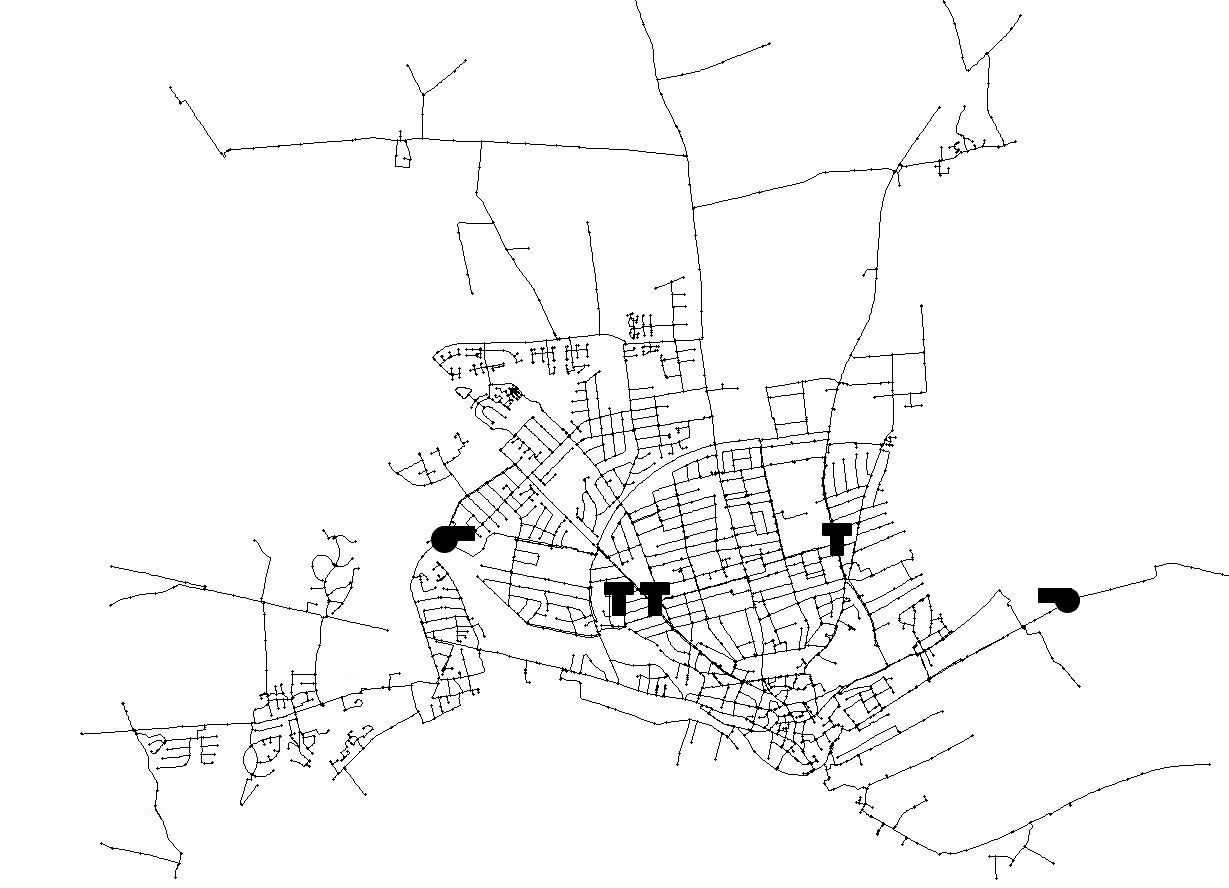
\includegraphics[width=\textwidth]{report/tikz/identification_map1}};
\node[black] at (11.4,4.75) {\footnotesize $\bm {\mathcal{W}_3}$};
\node[black] at (13.75,3.3) {\footnotesize $\bm {\mathcal{K}_2}$};
\node[black] at (4.7,4.65) {\footnotesize $\bm {\mathcal{K}_1}$};
\node[black] at (8.4,1) {\footnotesize $\bm {\mathcal{W}_2}$};
\node[black] at (6.8,1) {\footnotesize $\bm {\mathcal{W}_1}$};
\draw [-latex][thick](8.05,3.2) -- (8.4,1.35);
\draw [-latex][thick](7.55,3.2) -- (6.8,1.35);
\end{tikzpicture}

%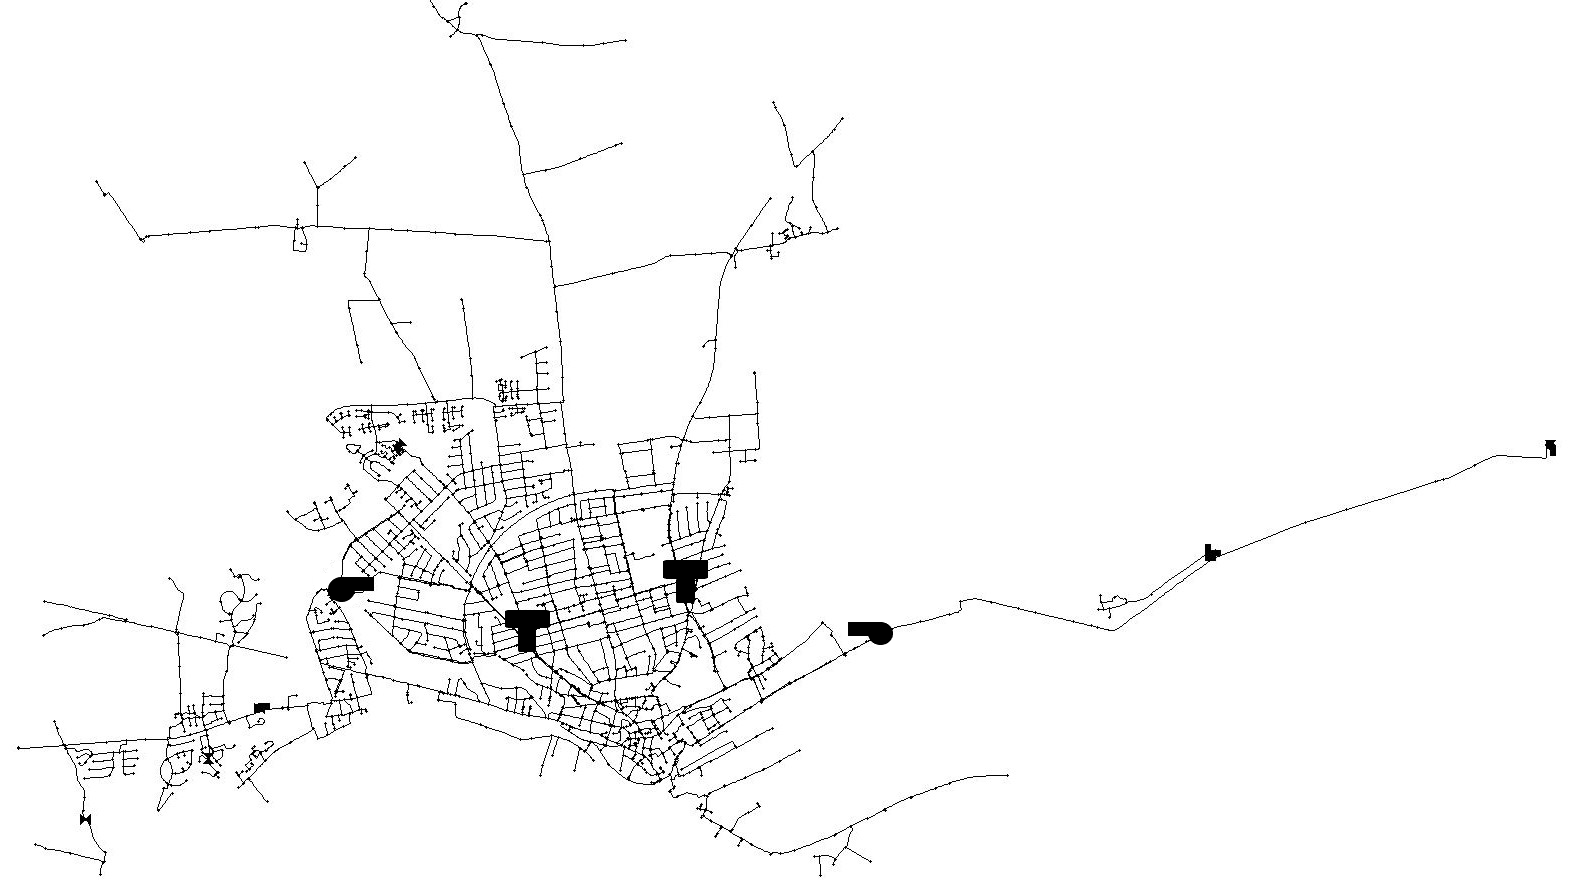
\includegraphics[width=0.95\textwidth]{report/pictures/verdo_pic3}
\caption{The network map with the corresponding WTs and pumping stations.}
\label{fig:simplified_network_identification}
\end{figure}
\vspace{-3mm}


 %Total consumptions
 \begin{figure}[H]
 \centering
 %\hspace{0mm}
 %
\includegraphics[width=0.35\textwidth]{report/pictures/missingfigure}
 % This file was created by matlab2tikz.
%
%The latest updates can be retrieved from
%  http://www.mathworks.com/matlabcentral/fileexchange/22022-matlab2tikz-matlab2tikz
%where you can also make suggestions and rate matlab2tikz.
%
\definecolor{mycolor1}{rgb}{0.00000,0.44700,0.74100}%
%
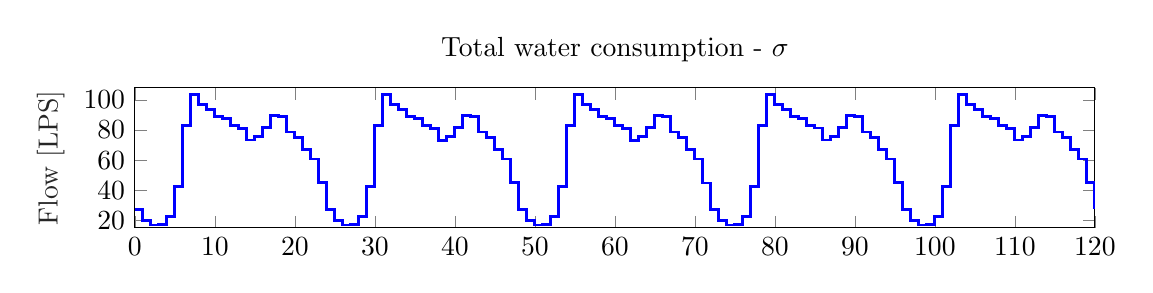
\begin{tikzpicture}

\begin{axis}[%
width=4.8in,
height=0.7in,
at={(0.888in,0.432in)},
scale only axis,
xmin=0,
xmax=120,
%xlabel style={font=\color{white!15!black}},
%xlabel={Time [h]},
ymin=15,
ymax=108,
ylabel style={font=\color{white!15!black}},
ylabel={Flow  [LPS]},
axis background/.style={fill=white},
title style={},
title={Total water consumption - $\sigma$}
]
\addplot[const plot, color=blue, line width=1pt, forget plot] table[row sep=crcr] {%
0	27.39\\
1	19.81\\
2	16.93\\
3	17.32\\
4	22.81\\
5	42.61\\
6	82.99\\
7	103.44\\
8	97.07\\
9	93.68\\
10	88.91\\
11	87.69\\
12	82.95\\
13	81.27\\
14	73.3\\
15	75.84\\
16	81.56\\
17	89.81\\
18	88.84\\
19	78.71\\
20	75.05\\
21	66.84\\
22	60.75\\
23	44.89\\
24	27.4\\
25	19.81\\
26	16.92\\
27	17.32\\
28	22.81\\
29	42.61\\
30	82.99\\
31	103.44\\
32	97.08\\
33	93.69\\
34	88.91\\
35	87.7\\
36	82.94\\
37	81.27\\
38	73.29\\
39	75.84\\
40	81.55\\
41	89.83\\
42	88.85\\
43	78.69\\
44	75.05\\
45	66.84\\
46	60.74\\
47	44.89\\
48	27.39\\
49	19.82\\
50	16.93\\
51	17.32\\
52	22.81\\
53	42.61\\
54	82.99\\
55	103.43\\
56	97.08\\
57	93.68\\
58	88.91\\
59	87.71\\
60	82.95\\
61	81.27\\
62	73.29\\
63	75.84\\
64	81.55\\
65	89.82\\
66	88.8500000000001\\
67	78.69\\
68	75.05\\
69	66.83\\
70	60.73\\
71	44.88\\
72	27.4\\
73	19.81\\
74	16.93\\
75	17.33\\
76	22.8\\
77	42.6\\
78	83\\
79	103.43\\
80	97.08\\
81	93.69\\
82	88.92\\
83	87.7\\
84	82.95\\
85	81.29\\
86	73.3\\
87	75.84\\
88	81.55\\
89	89.82\\
90	88.85\\
91	78.69\\
92	75.05\\
93	66.84\\
94	60.75\\
95	44.9\\
96	27.39\\
97	19.83\\
98	16.92\\
99	17.33\\
100	22.8\\
101	42.6\\
102	82.98\\
103	103.43\\
104	97.08\\
105	93.69\\
106	88.92\\
107	87.69\\
108	82.95\\
109	81.27\\
110	73.3\\
111	75.85\\
112	81.55\\
113	89.82\\
114	88.86\\
115	78.7\\
116	75.05\\
117	66.83\\
118	60.74\\
119	44.89\\
120	27.39\\
};
\end{axis}
\end{tikzpicture}% 
 \vspace{-2.5mm}
 %\caption{Consumption pattern in the identification.}
 \label{fig:sigma_id}
 \end{figure}
\vspace{-8mm}

 %Inlet flows
 \begin{figure}[H]
 \centering
 %\hspace{0mm}
 %
\includegraphics[width=0.35\textwidth]{report/pictures/missingfigure}
 % This file was created by matlab2tikz.
%
%The latest updates can be retrieved from
%  http://www.mathworks.com/matlabcentral/fileexchange/22022-matlab2tikz-matlab2tikz
%where you can also make suggestions and rate matlab2tikz.
%
\definecolor{mycolor1}{rgb}{0.00000,0.44700,0.74100}%
\definecolor{mycolor2}{rgb}{0.85000,0.32500,0.09800}%
%
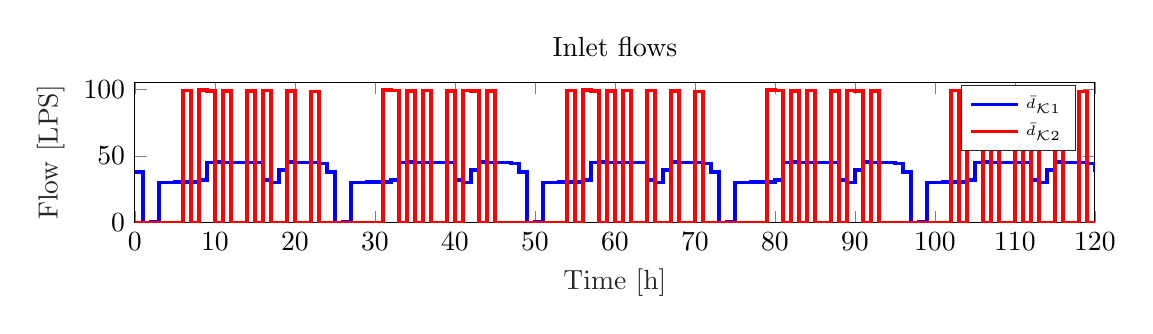
\begin{tikzpicture}

\begin{axis}[%
width=4.8in,
height=0.7in,
at={(0.758in,0.481in)},
scale only axis,
xmin=0,
xmax=120,
xlabel style={font=\color{white!15!black}},
xlabel={Time [h]},
ymin=0,
ymax=105,
ylabel style={font=\color{white!15!black}},
ylabel={Flow  [LPS]},
axis background/.style={fill=white},
title style={},
title={Inlet flows},
legend style={legend cell align=left, align=left, draw=white!15!black}
]
\addplot[const plot, color=blue, line width=1.2pt] table[row sep=crcr] {%
0	37.98\\
1	-0\\
2	0.59\\
3	30.03\\
4	30.03\\
5	30.33\\
6	30.33\\
7	30.33\\
8	31.8\\
9	45.05\\
10	45.34\\
11	45.05\\
12	44.76\\
13	45.05\\
14	44.76\\
15	45.05\\
16	31.8\\
17	30.03\\
18	39.46\\
19	45.34\\
20	45.05\\
21	44.76\\
22	45.05\\
23	44.46\\
24	37.98\\
25	-0\\
26	0.59\\
27	30.03\\
28	30.03\\
29	30.33\\
30	30.33\\
31	30.33\\
32	31.8\\
33	45.05\\
34	45.34\\
35	45.05\\
36	44.76\\
37	45.05\\
38	44.76\\
39	45.05\\
40	31.8\\
41	30.03\\
42	39.46\\
43	45.34\\
44	45.05\\
45	44.76\\
46	45.05\\
47	44.46\\
48	37.98\\
49	-0\\
50	0.59\\
51	30.03\\
52	30.03\\
53	30.33\\
54	30.33\\
55	30.33\\
56	31.8\\
57	45.05\\
58	45.34\\
59	45.05\\
60	44.76\\
61	45.05\\
62	44.76\\
63	45.05\\
64	31.8\\
65	30.03\\
66	39.46\\
67	45.34\\
68	45.05\\
69	44.76\\
70	45.05\\
71	44.46\\
72	37.98\\
73	-0\\
74	0.59\\
75	30.03\\
76	30.03\\
77	30.33\\
78	30.33\\
79	30.33\\
80	31.8\\
81	45.05\\
82	45.34\\
83	45.05\\
84	44.76\\
85	45.05\\
86	44.76\\
87	45.05\\
88	31.8\\
89	30.03\\
90	39.46\\
91	45.34\\
92	45.05\\
93	44.76\\
94	45.05\\
95	44.46\\
96	37.98\\
97	-0\\
98	0.59\\
99	30.03\\
100	30.03\\
101	30.33\\
102	30.33\\
103	30.33\\
104	31.8\\
105	45.05\\
106	45.34\\
107	45.05\\
108	44.76\\
109	45.05\\
110	44.76\\
111	45.05\\
112	31.8\\
113	30.03\\
114	39.46\\
115	45.34\\
116	45.05\\
117	44.76\\
118	45.05\\
119	44.46\\
120	37.98\\
};
\addlegendentry{\tiny $\bar{d}_{\mathcal{K}1}$}

\addplot[const plot, color=red, line width=1.2pt] table[row sep=crcr] {%
0	0\\
1	0\\
2	0\\
3	0\\
4	0\\
5	0\\
6	99.18\\
7	0\\
8	99.3\\
9	98.74\\
10	0\\
11	98.71\\
12	0\\
13	0\\
14	98.63\\
15	0\\
16	98.82\\
17	0\\
18	0\\
19	98.6\\
20	0\\
21	0\\
22	98.41\\
23	0\\
24	0\\
25	0\\
26	0\\
27	0\\
28	0\\
29	0\\
30	0\\
31	99.38\\
32	98.95\\
33	0\\
34	98.68\\
35	0\\
36	99.16\\
37	0\\
38	0\\
39	98.55\\
40	0\\
41	99.14\\
42	98.62\\
43	0\\
44	98.54\\
45	0\\
46	0\\
47	0\\
48	0\\
49	0\\
50	0\\
51	0\\
52	0\\
53	0\\
54	99.15\\
55	0\\
56	99.3\\
57	98.73\\
58	0\\
59	98.71\\
60	0\\
61	99.18\\
62	0\\
63	0\\
64	98.76\\
65	0\\
66	0\\
67	98.58\\
68	0\\
69	0\\
70	98.4\\
71	0\\
72	0\\
73	0\\
74	0\\
75	0\\
76	0\\
77	0\\
78	0\\
79	99.38\\
80	98.94\\
81	0\\
82	98.68\\
83	0\\
84	99.15\\
85	0\\
86	0\\
87	98.54\\
88	0\\
89	99.15\\
90	98.62\\
91	0\\
92	98.55\\
93	0\\
94	0\\
95	0\\
96	0\\
97	0\\
98	0\\
99	0\\
100	0\\
101	0\\
102	99.17\\
103	0\\
104	99.3\\
105	98.74\\
106	0\\
107	98.71\\
108	0\\
109	0\\
110	98.64\\
111	0\\
112	98.76\\
113	0\\
114	0\\
115	98.59\\
116	0\\
117	0\\
118	98.4\\
119	0\\
120	0\\
};
\addlegendentry{\tiny $\bar{d}_{\mathcal{K}2}$}

\end{axis}
\end{tikzpicture}% 
 \vspace{-2.5mm}
 \caption{Inlet flows of the two pumping stations.}
 \label{fig:dk_12}
 \end{figure}
 \vspace{-3mm}